\section{Grundbegriffe}

\textbf{Informationsgehalt} eines Ereignisses $I_i$ hängt von der Wahrscheinlichkeit $p_i$ ab, mit der das Ereignis eintritt:
$$I = \text{ld}(1/p_i) \quad\text{[bit]}$$

$\rightarrow$ Seltene Ereignisse haben danach einen hohen, häufige Ereignisse einen geringen Informationsgehalt
\begin{center}
	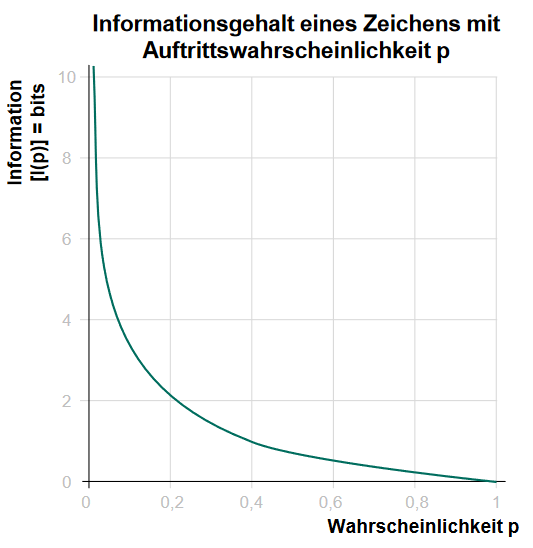
\includegraphics[width=0.4\textwidth]{images/informationsgehalt.png}
\end{center}

\textbf{Entropie} beschreibt das Maß der Unordnung bei Zeichen in einem Text:
$$H(I)=\sum (p_j\cdot\text{ld}(1/p_j))\quad \text{[bits/Zeichen]}$$

$\rightarrow$ Je gleichmäßiger die Zeichen verteilt sind, desto größer ist die Entropie und desto mehr Platz wird auch für die Kodierung benötigt

\begin{center}
	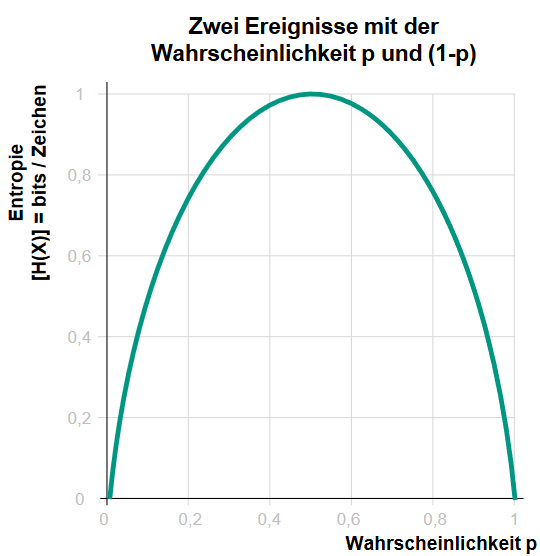
\includegraphics[width=0.4\textwidth]{images/entropie.png}
\end{center}

\textbf{Semiotik} ist die Wissenschaft von den Zeichenprozessen in Kultur und Natur
\begin{itemize}
	\item Zeichen vermitteln Informationen aller Art in Zeit und Raum
	\item Zeichen bzw. Signale beschreiben nur das, was nach vorgegebenen Regeln codiert werden kann (\textbf{Syntaktik})
	\item Bedeutung von Zeichen wird als \textbf{Semantik} bezeichnet
	\item Beeinflussung des Verhaltens des Empfängers durch Zeichen wird als \textbf{Pragmatik} bezeichnet
\end{itemize}

\textbf{Morris’ semiotisches Dreieck}:
\begin{center}
	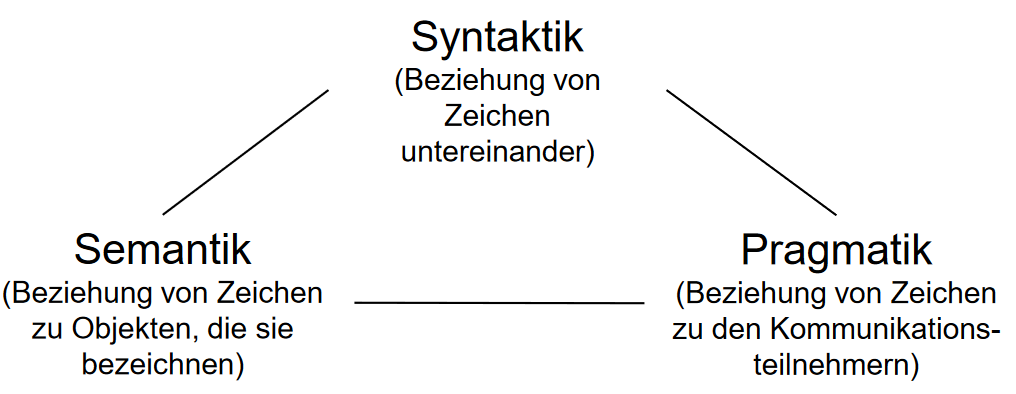
\includegraphics[width=0.6\textwidth]{images/semiotisches Dreieck.png}
\end{center}

\textbf{Zeichen} sind etwas Sichtbares oder Hörbares, das auf etwas aufmerksam macht. Durch die Aneinanderreihung von Zeichen entsteht eine Zeichenfolge oder ein Zeichenkomplex

Ein \textbf{Datum} wird allgemein als gegebener Gegenstand oder Sachverhalt bezeichnet. \textbf{Daten} sind Zuordnungen von Zeichen zu Objekten und Sachverhalten der Wirklichkeit.

Die Weitergabe von Bedeutung tragenden Zeichen oder Daten wird als \textbf{Nachricht} bezeichnet.

Weitergegebene Daten in Form von Nachrichten werden zu \textbf{Information}, wenn sie beim Empfänger eine Handlung auslösen oder ein beabsichtigtes Nichthandeln bewirken
\begin{itemize}
	\item \textbf{Ziel}: So viel Information wie möglich mit so wenig Zeichen wie möglich übermitteln
	\item Teil der Nachricht, der ohne Verlust an Information weggelassen werden kann, wird als \textbf{Redundanz} bezeichnet
	\item Nachricht, die für den Empfänger keine Information enthält, ist vollständig redundant und ihr Informationsgehalt ist somit Null
\end{itemize}

\textbf{Eigenschaften von Daten}:
\begin{itemize}
	\item können ohne Abnutzung mehrmals zur Informationsproduktion verwendet werden
	\item Reproduzierbar
	\item können auf einfache Weise kopiert und mit Lichtgeschwindigkeit transportiert werden
	\item Wert von Daten hängt von der Art ihrer Verwendung ab
\end{itemize}
\pagebreak

\textbf{Herausforderungen der Informationsproduktion}:
\begin{itemize}
	\item \textbf{Informationsverluste} durch das Löschen weniger relevant eingeschätzter Daten sowie durch deren Aggregation und Komprimierung
	\item \textbf{Informationsüberlastung}, wenn zu viele Daten zu einer Verschlechterung der kognitiven Wahrnehmung über die Sachverhalte führen, die durch sie beschrieben werden. Bei starker Überflutung spricht man von \textbf{Informationsschock}.
	\item \textbf{Informationspathologien} durch Mängel bei der Informationsproduktion, wenn produzierbare
	Information nicht produziert, beschaffbare nicht beschafft und vorhandene falsch oder nicht verwendet wird
	\item \textbf{Informationsverzerrung} durch intrapersonelles, meist unbewusstes, selektives Wahrnehmen von Information und das interpersonelle, meist bewusste Durchsetzen individueller Anschauungen. Bewusste Verzerrung führt zu \textbf{Informationsmissbrauch}
\end{itemize}

\textbf{Wissenspyramide}: 
\begin{center}
	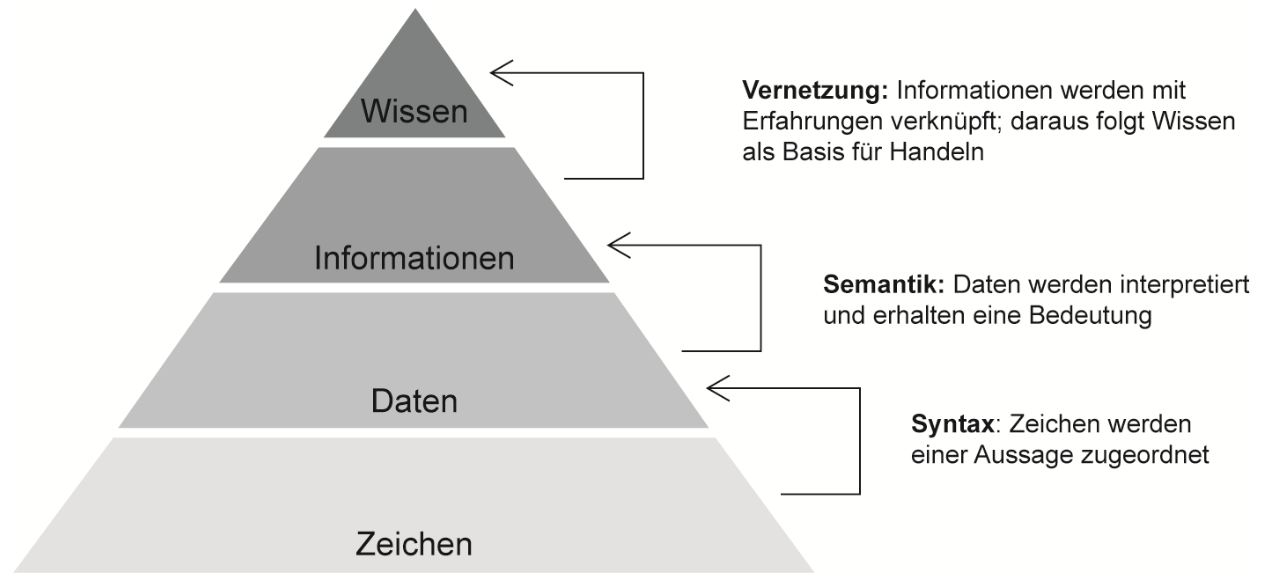
\includegraphics[width=0.8\textwidth]{images/wissenspyramide.png}
\end{center}

\textbf{Nonaka Takeuchi Modell des Wissensmanagements (SECI-Modell)}:
\begin{center}
	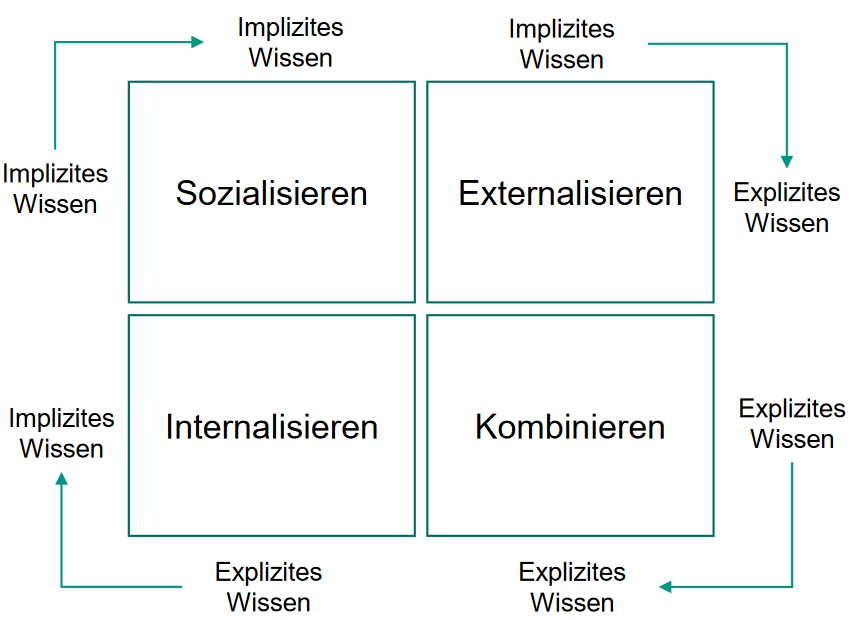
\includegraphics[width=0.5\textwidth]{images/nonaka.png}
\end{center}

\pagebreak
\textbf{Kommunikation} ist die Beziehung, die zwischen Menschen, Lebewesen, maschinellen Systemen oder Geräten durch Austausch von Nachrichten entsteht $\rightarrow$ \textbf{Ziel}: Sender will Empfänger informieren

\textbf{Sender-Empfänger-Kommunikationsmodell}:
\begin{center}
	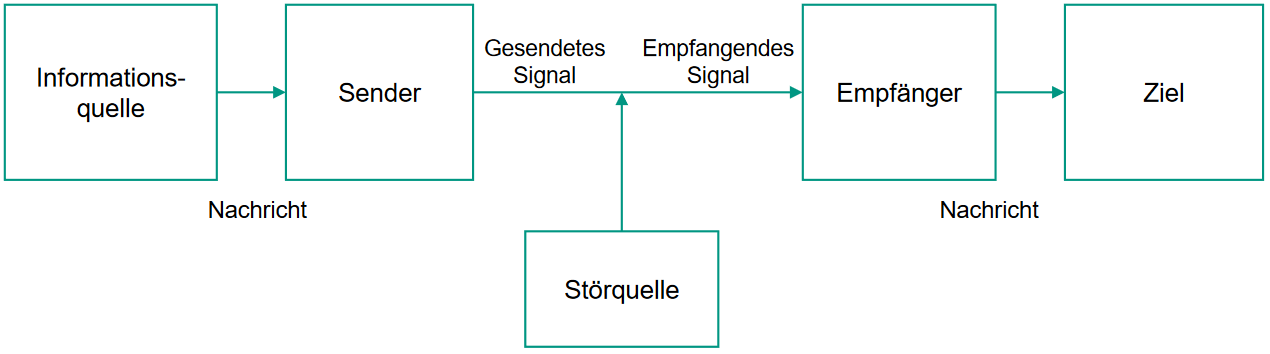
\includegraphics[width=0.8\textwidth]{images/sue-modell.png}
\end{center}

\textbf{Ebenen der Kommunikation}:
\begin{center}
	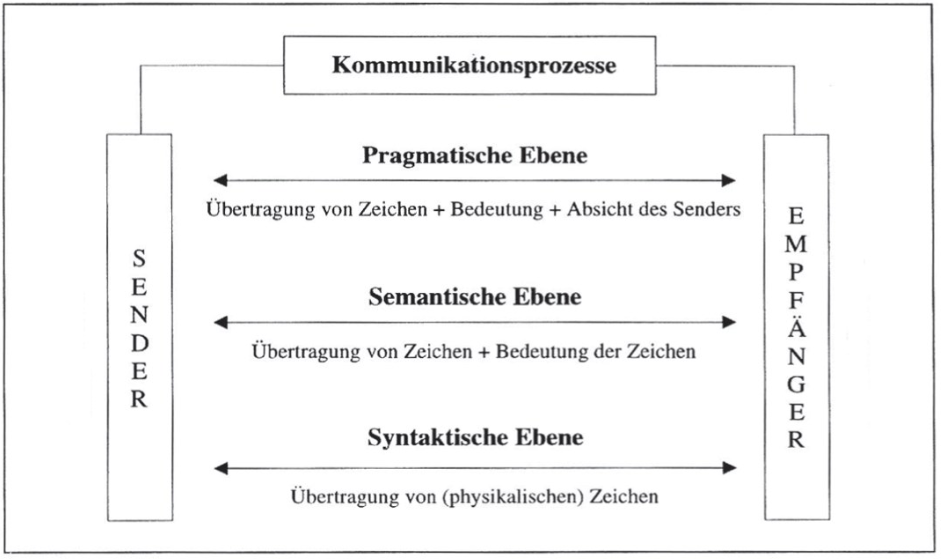
\includegraphics[width=0.8\textwidth]{images/ebenen.png}
\end{center}

\textbf{Informationsbedarf} bezeichnet die Art, Menge und Beschaffenheit von Information, die zur Erfüllung einer Aufgabe benötigt wird

\textbf{Informationsbedürfnis} bezeichnet das Verlangen nach Information aus der Sicht der Aufgabenträger

\textbf{Informationsangebot} bezeichnet die Art, Menge und Beschaffenheit von Information, welche Aufgabenträgern zur Verfügung gestellt wird

\textbf{Informationsnachfrage} beschreibt welche Information zur Aufgabenerfüllung in einer konkreten Handlungssituation vom Aufgabenträger nachgefragt wird

Schnittmenge von Informationsbedarf, -bedürfnis, -nachfrage und -angebot wird als \textbf{Informationsstand} bezeichnet
\begin{itemize}
	\item Wenn Informationsnachfrage größer als das Informationsangebot ist, wird dies \textbf{Informationsdefizit} genannt
	\item Wenn Informationsangebot größer als die Informationsnachfrage ist, wird dies \textbf{Informationsüberschuss} genannt
\end{itemize}
\begin{center}
	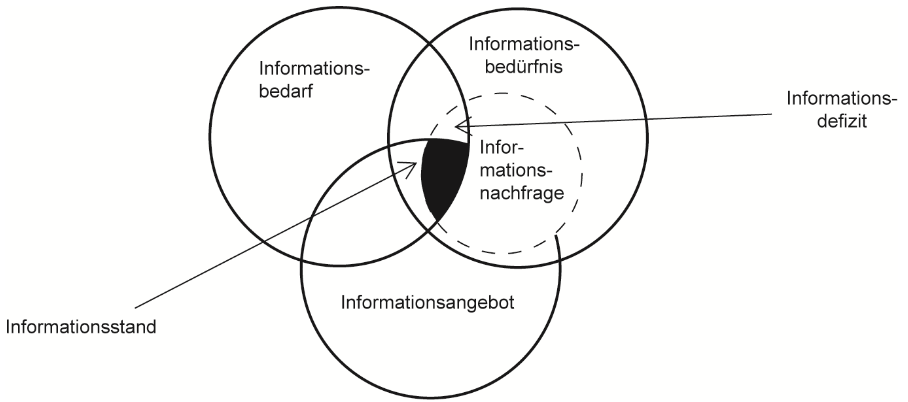
\includegraphics[width=0.8\textwidth]{images/infodefizit.png}
\end{center}

\section{Gegenstandsbereich und Typisierung}
\textbf{Technik} beschreibt 1) das Regeln folgende und Ziele anstrebende Handeln und Denken (Arbeitstechnik) und 2) vom Menschen geschaffene Geräte und Maschinen (Sachtechnik).

\textbf{Informations- und Kommunikationstechnik} (IKT) ist die Technik für Information und Kommunikation

\textbf{System} meint den ganzheitlichen Zusammenhang von Elementen, die voneinander abhängig sind, ineinandergreifen oder zusammenwirken
\begin{itemize}
	\item Verbindungen, die durch die Abgrenzung des Systems von seiner Umwelt entstehen, heißen \textbf{Schnittstellen}
	\item Jedes System ist Teil eines übergeordneten Systems und jedes System kann in Teilsysteme zerlegt werden
\end{itemize}
\begin{center}
	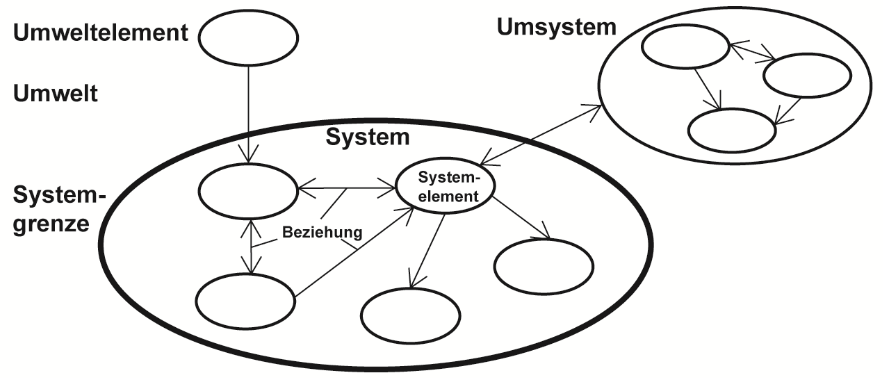
\includegraphics[width=0.7\textwidth]{images/system.png}
\end{center}

\pagebreak
\textbf{Systemeigenschaften}:
\begin{itemize}
	\item Offenheit versus Geschlossenheit: Offenheit ist die Eigenschaft eines Systems, über seine Elemente mit seiner Umwelt in Beziehung zu stehen
	\item Komplexität versus Einfachheit: Komplexität ist die Eigenschaft eines Systems, die durch die Anzahl seiner Elemente und durch die Anzahl der Beziehungen zwischen den Elementen gegeben ist
	\item Kompliziertheit versus Einfachheit: Kompliziertheit ist die Eigenschaft eines Systems, die durch die Anzahl der Elemente und deren Verschiedenartigkeit gegeben ist
	\item Dynamik versus Statik: System, in dem sich die Zustände der Elemente oder die der Beziehungen im Zeitablauf verändern, heißt dynamisches System
	\item Zweckorientiert und zielorientiert: Zwecke beschreiben, welche Aufgaben sie erfüllen sollen, Ziele beschreiben die Qualität, mit der die Zwecke erreicht werden sollen
\end{itemize}

\textbf{Sozio-Technische Systeme}
\begin{itemize}
	\item \textbf{Soziales Subsystem}: Individuen, Gruppen, Organisationen, Märkte
	\item \textbf{Technologisches Subsystem}: Software, Hardware,  Technische Infrastruktur
\end{itemize}

\textbf{Erkenntnisobjekte der Wirtschaftsinformatik}: Informationsfunktion, Informationssystem, Informationsinfrastruktur

\textbf{Informationsfunktion} umfasst die betrieblichen Aufgaben, deren Zweck die Produktion von Information ist und deren Bereitstellung durch Kommunikation erfolgt (Informationsaufgaben)
$\rightarrow$ Richtige Informationen, Zeitpunkt, Menge, Ort, Qualität

\textbf{Informationssysteme} sind Mensch/Aufgabe/Technik-Systeme, kurz gesagt MAT-Systeme
\begin{itemize}
	\item \textbf{Menschen} erfüllen Aufgaben und nutzen hierfür Informations- und Kommunikationstechniken
	\item \textbf{Aufgaben} stellen entweder Einzelprobleme oder ganze Problembereiche in Wirtschaft und Gesellschaft dar
\end{itemize}
\begin{center}
	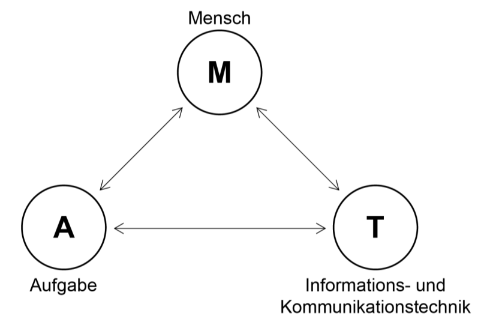
\includegraphics[width=0.4\textwidth]{images/mat.png}
\end{center}

\textbf{Informationsinfrastrukturen} sind organisatorische Gesamtheiten von Informationssystemen in Wirtschaft und Verwaltung, deren Verfügbarkeit und Anwendung Voraussetzung für Informationsproduktion und für Kommunikation im Unternehmen ist

\textbf{Typisierung nach Technik}:
\begin{center}
	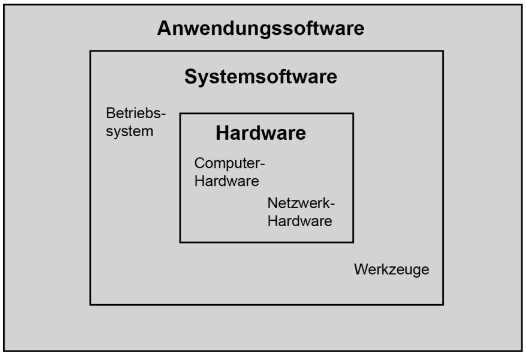
\includegraphics[width=0.5\textwidth]{images/typisierung-technik.png}
\end{center}

\textbf{Aufbau Anwendungssysteme}:
\begin{center}
	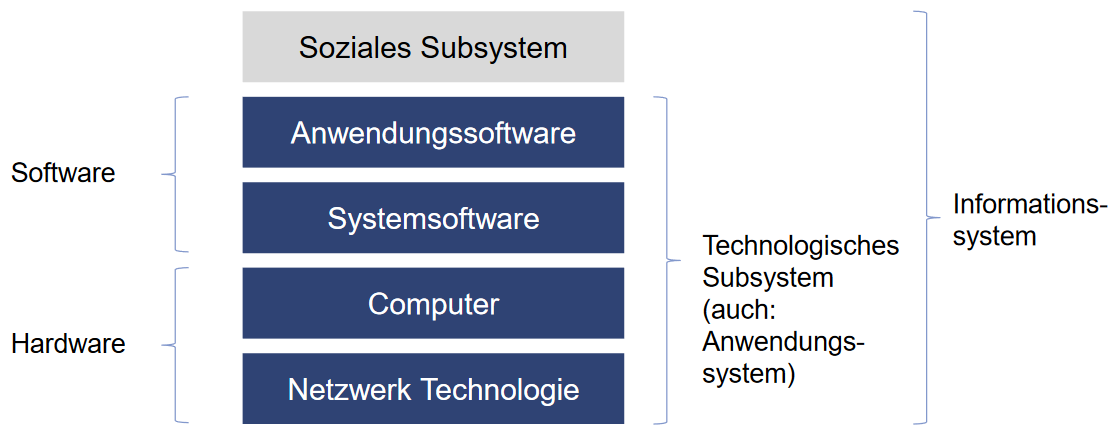
\includegraphics[width=0.7\textwidth]{images/anwendungssysteme.png}
\end{center}

\textbf{Unterscheidung von Anwendungssoftware}:
\begin{itemize}
	\item \textbf{Produktsoftware}: Standard-Software: wird von einem Software-Unternehmen verkauft, Geteilte Entwicklungskosten, Etablierte Best-practices, Vorschau möglich, Referenzimplementierung verfügbar
	\item \textbf{Individualsoftware}: Maßgeschneiderte Software: spezifische Entwicklung durch Dienstleister oder in-house, Wettbewerbsvorteil, Unternehmensspezifische Änderungen möglich, Unabhängigkeit vom Software-Lieferanten, Verwendete Firmenterminologie, weniger Schulungsaufwand
\end{itemize}

\textbf{Typisierung nach Mensch}: Mittels Personas können Systeme entlang von Nutzergruppen klassifiziert werden

\pagebreak
\textbf{Typisierung nach Aufgaben:}
\begin{center}
	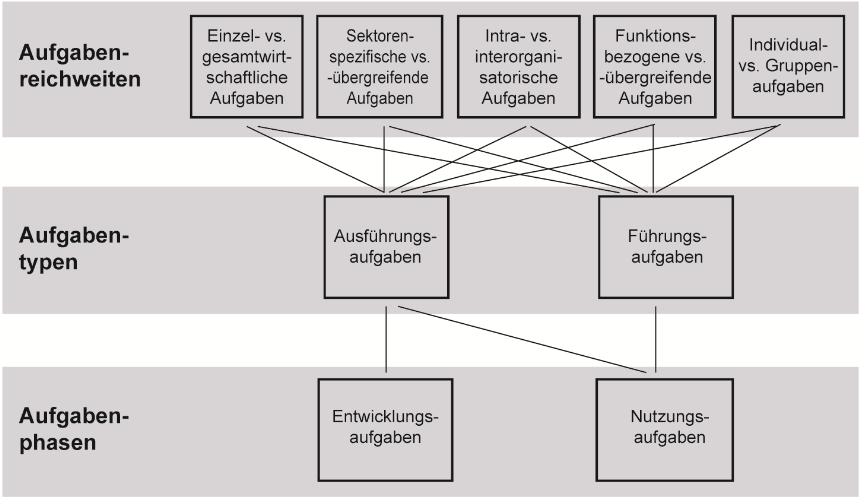
\includegraphics[width=0.7\textwidth]{images/typisierung-aufgaben.png}
\end{center}

\section{Digitale Organisation - Grundlagen}
\textbf{Unternehmen in der marktwirtschaftlichen Wirtschaftsordnung}:
\begin{itemize}
	\item \textbf{Organisationen} sind (1) soziale Einheiten, die (2) zielorientiert sind, (3) als bewusst strukturierte und koordinierte Aktivitätssysteme konzipiert sind und (4) mit dem externen Umfeld verbunden sind
	\item \textbf{Privatwirtschaftliche Unternehmen} sind primär gewinnorientierte Organisationen
	\item \textbf{Aktivitätssysteme} müssen so konzipiert werden, dass Verkaufswert höher ist als die Kosten
\end{itemize}

\textbf{Wertschöpfungskette} stellt aufeinander aufbauende Aktivitäten dar, die zur Herstellung eines Gutes oder
einer Dienstleistung erbracht werden

\textbf{Markttransaktion} ist die bilaterale Abwicklung eines Geschäftsakts , wobei Verfügungsrechte an
Gütern von einem Verkäufer zu einem Käufer übertragen werden. Verschiedene Transaktionsphasen:
\begin{itemize}
	\item Informationsphase
	\item Vereinbarungsphase
	\item Abwicklungsphase
	\item Verkaufsfolgephase
\end{itemize}

\textbf{Transaktionskosten} sind Kosten, die durch Markttransaktionen verursacht werden. Sie entstehen nicht durch die Gütererstellung, sondern durch die Übertragung von Gütern von einem Marktteilnehmer zum anderen. $\rightarrow$ Höhe der Transaktionskosten kann die Wahl der Beschaffungs- und Vertriebswege sowie die Wahl der Marktpartner erheblich beeinflussen

\textbf{Lieferketten} sind übergreifende Wertschöpfungsketten, bei der die Glieder der Kette  durch geschäftliche Transaktionen verbunden sind

\textbf{Gestaltungsebenen in Organisationen}:
\begin{center}
	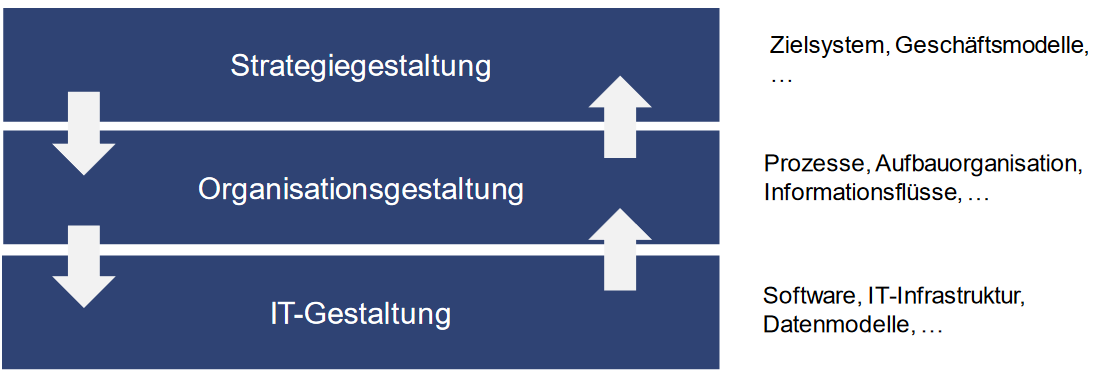
\includegraphics[width=0.7\textwidth]{images/gestaltungsebenen.png}
\end{center}

\textbf{Strukturelle Dimensionen der Organisationsgestaltung}:
\begin{center}
	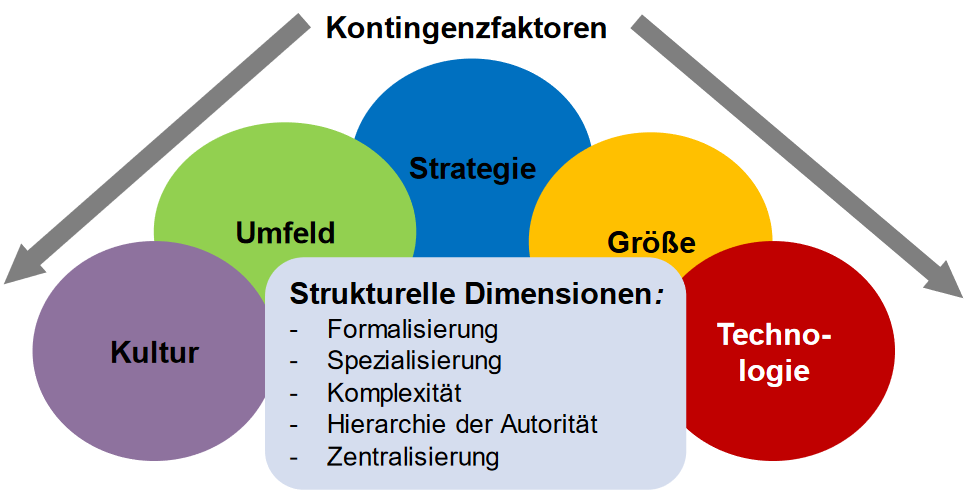
\includegraphics[width=0.7\textwidth]{images/organisationsgestaltung.png}
\end{center}
\begin{itemize}
	\item \textbf{Formalisierung} ist der Grad zu welchem Rollen strukturiert sind und die Aktivitäten der Mitarbeiter durch Regeln und Prozesse vorgegeben sind
	\item \textbf{Spezialisierung} ist der Grad zu welchem die Aufgaben in einzelne Schritte aufgeteilt werden 
	\item \textbf{Komplexität} bezieht sich auf die Anzahl der verschiedenen Abteilungen oder Aktivitäten innerhalb des Unternehmens. Komplexität kann in drei Dimensionen gemessen werden: vertikal, horizontal und räumlich.
	\item \textbf{Hierarchie der Autorität} beschreibt die Berichts- und Rechenschaftswege, sowie die den Bereich der Kontrolle und Weisungsbefugnis für jeden Manager
	\item \textbf{Zentralisierung} meint das hierarchische Level auf welchem die Autorität für das Fällen von Entscheidungen zugeordnet ist
\end{itemize}

\pagebreak
\textbf{Verschiedene Organisationsstrukturen}:
\begin{center}
	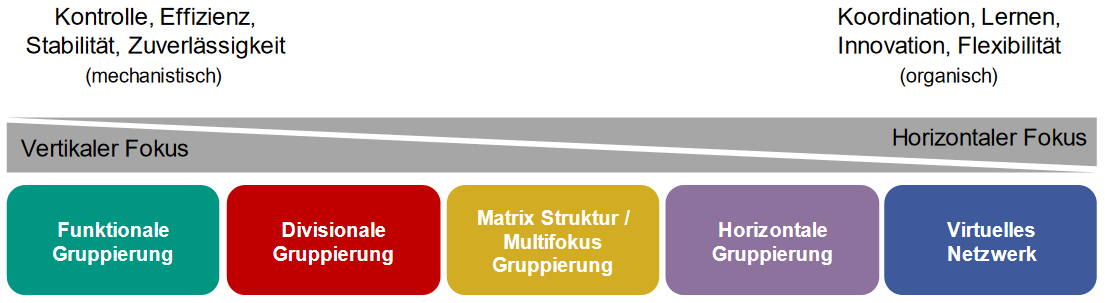
\includegraphics[width=0.8\textwidth]{images/organisationsstrukturen.png}
\end{center}

\textbf{Prozess} ist eine Abfolge von  miteinander verbundenen Aktivitäten, die in jeder Phase Ressourcen verbrauchen, um Inputs in Outputs umzuwandeln. Diese Outputs dienen dann als Input für die nächste Stufe, bis ein
bekanntes Ziel oder Endergebnis erreicht ist
\begin{center}
	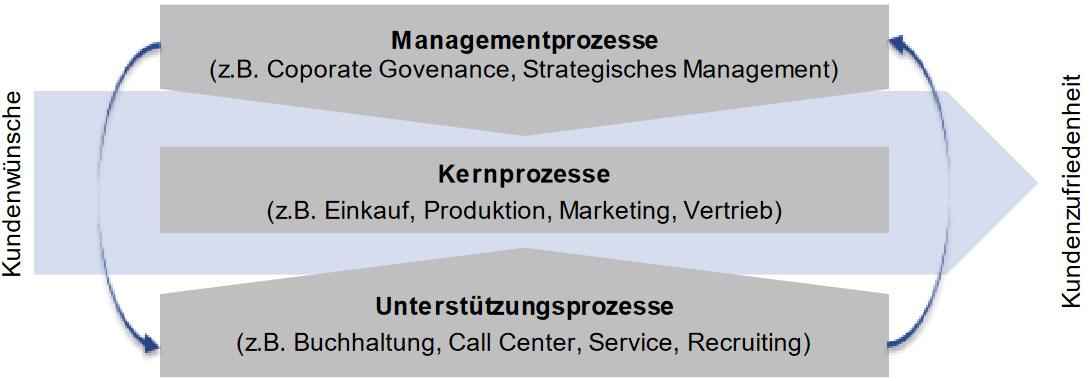
\includegraphics[width=0.7\textwidth]{images/prozess.png}
\end{center}

\textbf{Transaktion im engeren Sinne} ist ein logisch abgeschlossener Vorgang auf der Anwendungsebene, der eine
zusammengehörige Einheit darstellt, die vollständig oder gar nicht durchgeführt werden soll

\textbf{Stammdaten} sind wichtige Grunddaten eines Unternehmens, die über einen gewissen Zeitraum nicht verändert und nur periodisch aktualisiert werden 

\textbf{Transaktionsdaten} fallen im Rahmen der Durchführung von Transaktionen an 

\textbf{Betriebliches Informationssystem} unterstützt die Leistungsprozesse und Austauschbeziehungen innerhalb eines Betriebs sowie zwischen dem Betrieb und seiner Umwelt

\textbf{Vergleich von betrieblichen Informationssystemen}:
\begin{center}
	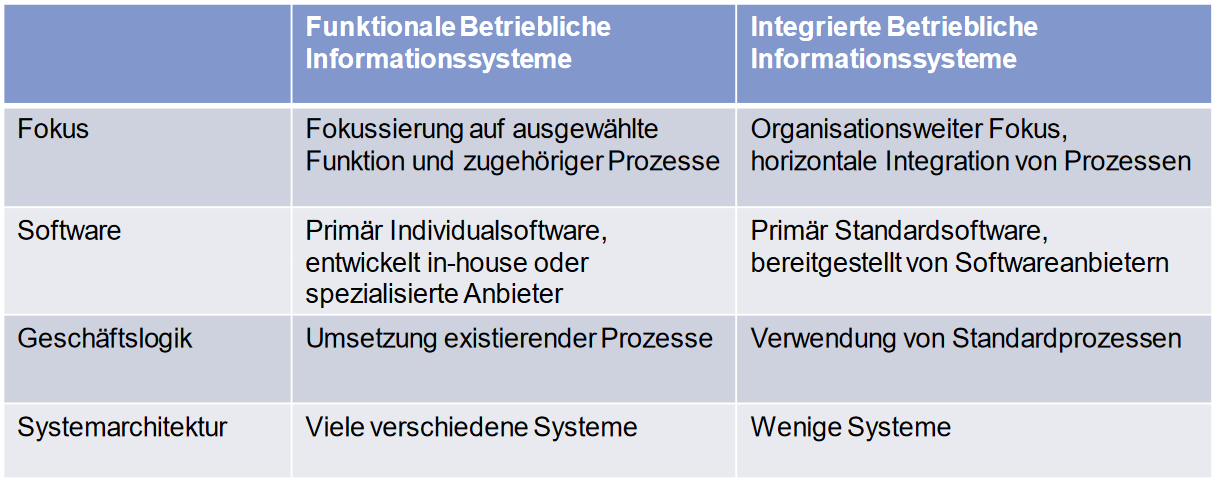
\includegraphics[width=0.8\textwidth]{images/informationssysteme.png}
\end{center}

\textbf{Integration} beschreibt die Verknüpfung von Elementen bzw. Subsystemen zu einem System

\textbf{Vertikale und Horizontale Integration}:
\begin{center}
	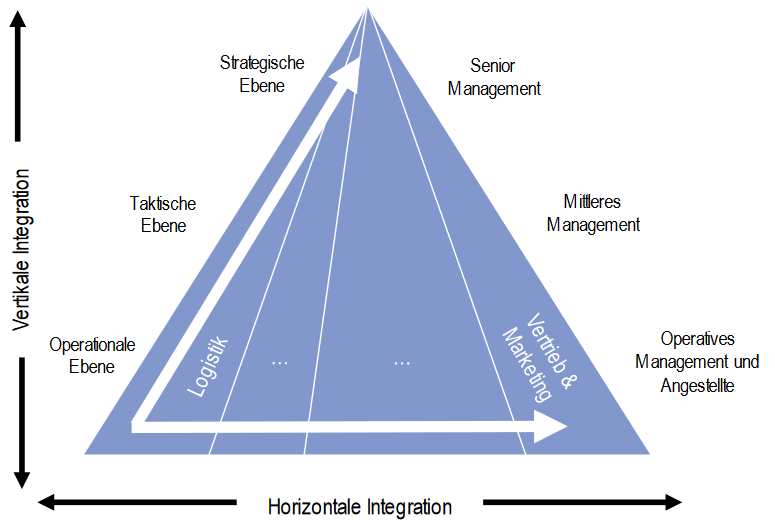
\includegraphics[width=0.6\textwidth]{images/integration.png}
\end{center}
\begin{itemize}
	\item Vertikal integriertes Informationssystem verknüpft Teilsysteme des gleichen Funktionsbereichs auf verschiedenen Stufen
	\item Horizontal integriertes Informationssystem verbindet Teilsysteme aus unterschiedlichen Funktionsbereichen auf einer Ebene
\end{itemize}

\textbf{Klassen unterschiedlicher betrieblicher Informationssysteme}:
\begin{itemize}
	\item Managementunterstützungssysteme, inkl. Planungs- und Kontrollsystem
	\item Büroinformationssysteme
	\item Operative Informationssysteme 
\end{itemize}

\textbf{Operatives Informationssystem} unterstützt die alltäglichen betrieblichen Leistungsprozesse mithilfe von
betrieblicher Anwendungssoftware

\textbf{Büroinformationssysteme} stellen Funktionen zum Erstellen von Textdokumenten, Tabellen, Zeichnungen oder Präsentationen sowie zur Unterstützung der Zusammenarbeit und Kommunikation oder Aufgaben des Dokumentationswesens und des Wissensmanagements

\textbf{Planungssystem} unterstützt die Führungskräfte eines Betriebs bei ihren Planungsaufgaben. Ein \textbf{Kontrollsystem} dient zur Überwachung der Einhaltung der Pläne durch Soll-Ist-Vergleiche und Hinweise auf notwendige Korrekturmaßnahmen $\rightarrow$ Zusammengefasst: \textbf{Managementunterstützungssysteme}

\textbf{Zwischenbetriebliches Informationssystem} verbindet die Informationssysteme zweier oder mehrerer Betriebe

\textbf{Konsumenteninformationssystem} dient zur Interaktion mit vornehmlich privaten Kunden bzw.
Interessenten, mit denen unter Umständen bisher nur sehr wenige geschäftliche Kontakte bestanden

\section{Digitale Organisationen - ERP und ZB Systeme}
\textbf{ERP-System} ist ein aus mehreren Komponenten bestehendes integriertes betriebliches Anwendungssystem, welches die operativen Prozesse in allen wesentlichen betrieblichen Funktionsbereichen unterstützt.
\begin{itemize}
	\item Integration durch Datenbanksystem $\rightarrow$ keine Datenredundanzen, gleichzeitiger, transaktionaler Zugriff, gemeinsame Sicht auf Daten
\end{itemize}

\textbf{Finanzierung} fokussiert sich auf die Bereitstellung und zielgerichtete Verwendung finanzieller Mittel

\textbf{Rechnungswesen} ist die systematische Erfassung der durch die betrieblichen Leistungsprozesse entstehenden Transaktionen und die Überwachung der Wirtschaftlichkeit

\textbf{Finanzbuchhaltung} zeichnet alle finanziellen Geschäftsvorfälle auf. Sie wird nach gesetzlichen Vorschriften erstellt, dient der Dokumentation, der Gewinnermittlung und der Steuerbemessung, und bildet die Basis betriebswirtschaftlicher Erfolgsrechnungen $\rightarrow$ Erfassung erfolgt im ERP-System auf Konten

Bilanz und G+V werden aus dem \textbf{Hauptbuch} erstellt. Im Hauptbuch werden alle Buchungen zusammengeführt

\textbf{Nebenbücher} werden bei wichtigen Vermögens- werten geführt, um eine detaillierte Verrechnung darstellen zu können

\textbf{Kostenarten-/Kostenstellen-/Kostenträgerrechnung}: 
\begin{center}
	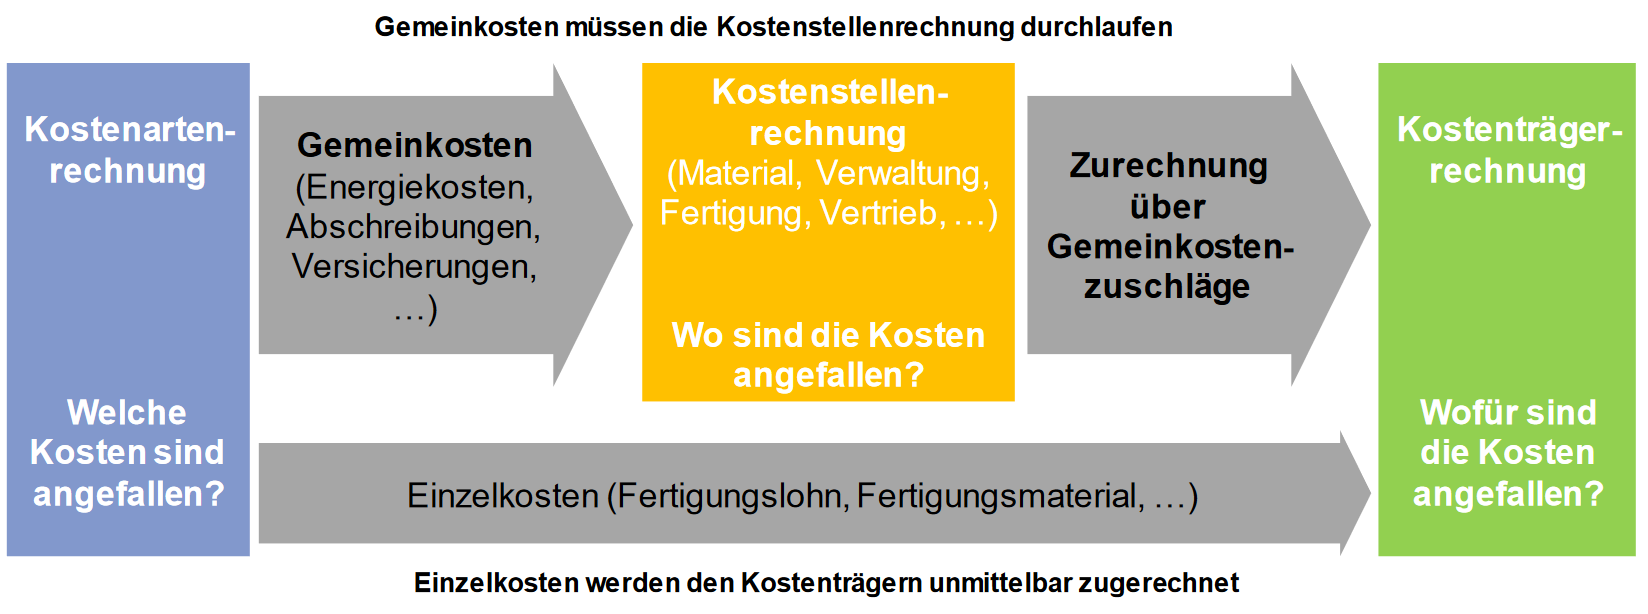
\includegraphics[width=0.8\textwidth]{images/kkk.png}
\end{center}

Unter \textbf{Personalwirtschaft oder Personalwesen} versteht man die Bereitstellung und den zielgerichteten Einsatz von Mitarbeitern in Betrieben
\begin{itemize}
	\item Wirtschaftliches Ziel: Finden von bestgeeigneten Mitarbeitern
	\item Soziales Ziel: Bestmögliche Arbeitsverhältnisse für die Mitarbeiter
\end{itemize}

Unter \textbf{Materialwirtschaft} versteht man die Planung, Steuerung, Verwaltung und Kontrolle der Materialbestände und -bewegungen innerhalb eines Betriebs und zwischen dem Betrieb und seinen Marktpartnern
\begin{itemize}
	\item Hauptaufgaben: Einkauf, Lagerhaltung, Disposition und Rechnungsprüfung
	\item \textbf{Logistik} umfasst neben der Materialwirtschaft auch den Transport, den Zwischenwerksverkehr, Warenumschlagsstellen, die Instandhaltung und die Entsorgung
\end{itemize}

\textbf{Produktionsplanungs- und Steuerungssystem} ist ein Anwendungssoftwaresystem, das die operative Produktionsplanung und -steuerung unterstützt

Unter \textbf{Vertrieb} wird die Abwicklung des Verkaufs und der damit verbundenen operativen Prozesse über die verschiedenen Absatzwege eines Betriebs verstanden

Ein \textbf{zwischenbetriebliches Informationssystem} verbindet die Informationssysteme zweier oder mehrerer Betriebe

\textbf{Einfache Wertschöpfungskette}: 
\begin{center}
	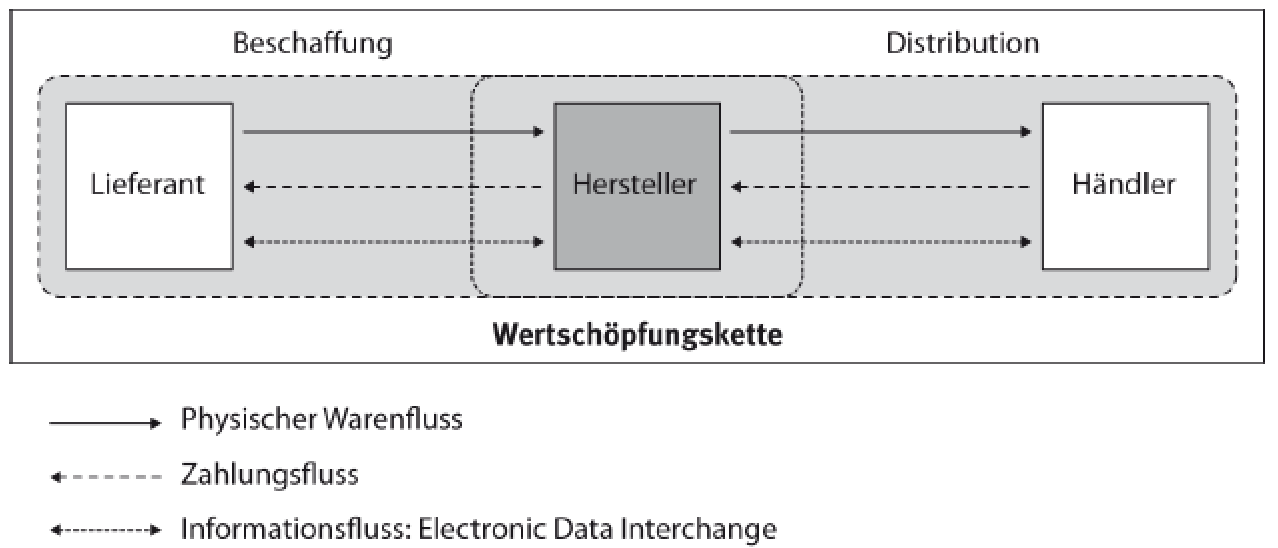
\includegraphics[width=0.8\textwidth]{images/sc.png}
\end{center}

\textbf{EDI (electronic data interchange)} ist der elektronische Datenaustausch über Geschäftstransaktionen zwischen Betrieben in strukturierten und einheitlichen Formaten

\textbf{Supply-Chain Management} ist das Management der Geschäftsprozesse der Versorgungskette vom ersten Rohstofflieferanten bis zum Endverbraucher

\textbf{Kooperationsmodelle des SCM}:
\begin{itemize}
	\item \textbf{Continuous Replenishment Program (CRP)}: Steuerung durch tatsächlicher Konsumentennachfrage bzw. dem prognostizierten Bedarf
	\item \textbf{Vendor-Managed Inventory (VMI)}: Übergabe der Verantwortung für Bestellungen und dem
	Bestandsmanagement an den Lieferanten
	\item \textbf{Just-in-Time (JIT)}: Koordination von Nachfrage und Angebot, sodass das Material genau dann eintrifft, wenn es benötigt wird
\end{itemize}

\section{Digitale Organisation - BIA und CRM Systeme}
\textbf{Business Intelligence \& Analytics (BI\&A)} sind Methoden, Technologien, Systeme und Anwendungen zur Analyse kritischer Geschäftsdaten mit dem Ziel einem Unternehmen zu helfen, das Geschäft und seinen Markt besser zu verstehen und zeitnahe Entscheidungen zu treffen

\textbf{Generische Architektur von Business Intelligence \& Analytics Systemen}:
\begin{center}
	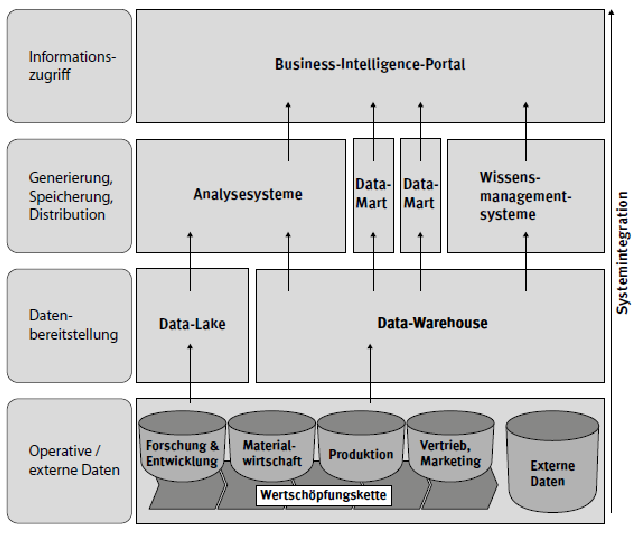
\includegraphics[width=0.6\textwidth]{images/bias.png}
\end{center}

\textbf{Data Warehouse} ist ein unternehmensweites Datenbanksystem, welches als logisch zentraler Speicher eine einheitliche und konsistente Datenbasis zur Entscheidungsunterstützung aller Bereiche und Ebenen bietet und losgelöst von den operativen Systemen betrieben wird

Ein \textbf{Data Mart} ist ein aggregierter Teilausschnitt aus dem Data-Warehouse, mit dem sich ein Großteil der Abfragen eines Funktionsbereichs oder einer Personengruppe einfach und schnell bedienen lässt
\begin{itemize}
	\item \textbf{Vorteile}: Verbesserte Leistung, erhöhte Flexibilität, geringer Abstimmungsaufwand, vereinfachter Zugriffsschutz
\end{itemize}

\pagebreak
\textbf{Data Warehouse Prozess}:
\begin{center}
	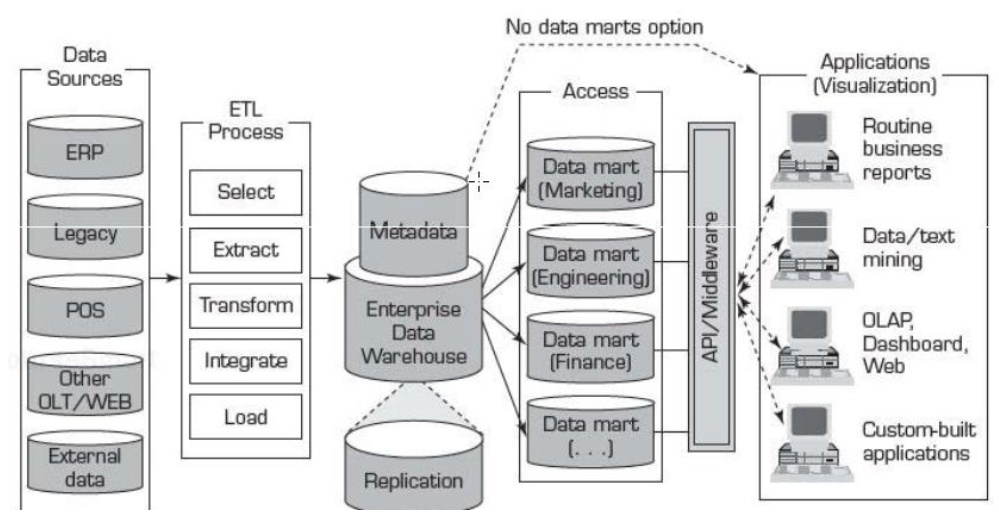
\includegraphics[width=0.8\textwidth]{images/dwp.png}
\end{center}

Betriebliche \textbf{Kennzahlen} sind charakterisierende Maßzahlen, die als bewusste Verdichtung der komplexen Realitat über zahlenmäßig erfassbare Sachverhalte, insbesondere über die Zielerreichung, informieren sollen
\begin{itemize}
	\item Unterscheidung zwischen \textbf{absoluten Kennzahlen} (z.B. Anzahl Mitarbeiter, Produkte usw.) und \textbf{relativen Kennzahlen} wie Umsatz pro Kunde oder pro Quartal
\end{itemize}

Ein \textbf{Kennzahlensystem} ist eine Zusammenstellung von einzelnen Kennzahlen, die in einer sachlich sinnvollen Beziehung zueinander stehen, einander ergänzen oder erklären und insgesamt auf ein gemeinsames, übergeordnetes Ziel ausgerichtet sind

\textbf{Multidimensionale Datenmodellierung}: 
\begin{center}
	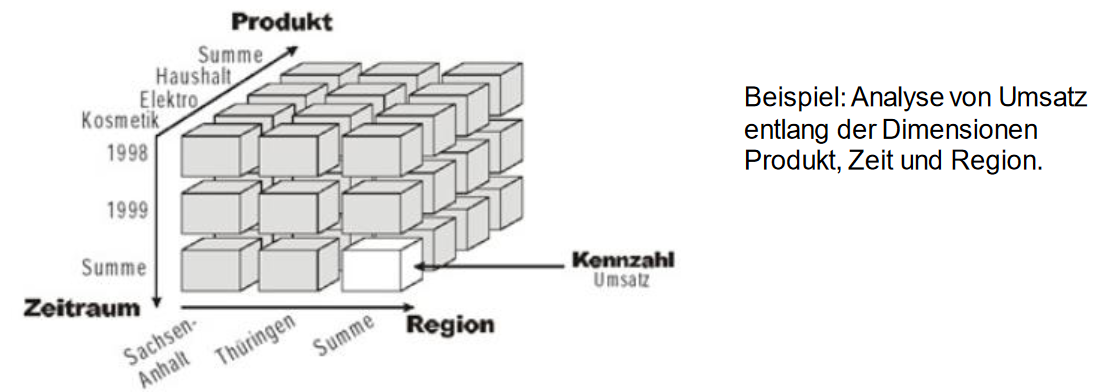
\includegraphics[width=0.8\textwidth]{images/mdd.png}
\end{center}

\textbf{Berichtswesen} stellt eine Verbindung zwischen Entstehungs- und Anwendungsort der Daten her. Es stellt für die unterschiedlichen Führungsebenen alle nötigen Informationen, die zur Entscheidungsfindung gebraucht werden, zur Verfügung

\textbf{Dashboard} ist ein Bericht, der Schlüsselkennzahlen zur Leistungsmessung aus unterschiedlichen Bereichen
eines Betriebs in einer konsolidierten, einheitlichen Bildschirmdarstellung meist grafisch darstellt 

\textbf{Big Data} bezeichnet große Datenmengen, die in unterschiedlicher Komplexität vorliegen, mit unterschiedlicher Geschwindigkeit erzeugt werden und unterschiedliche Grade an Mehrdeutigkeiten aufweisen

\textbf{Data Science} ist das Feld, welches sich mit der generalisierbaren Extraktion von Wissen aus Daten beschäftigt

\textbf{Data Lake} ist ein Datenbanksystem, in dem unternehmensrelevante Daten in ihrer Ursprungsform kostengünstig gespeichert und dann aufbereitet werden, wenn ein konkreter Bedarf besteht

\textbf{Vergleich: Business Intelligence vs. Business Analytics Systeme}:
\begin{center}
	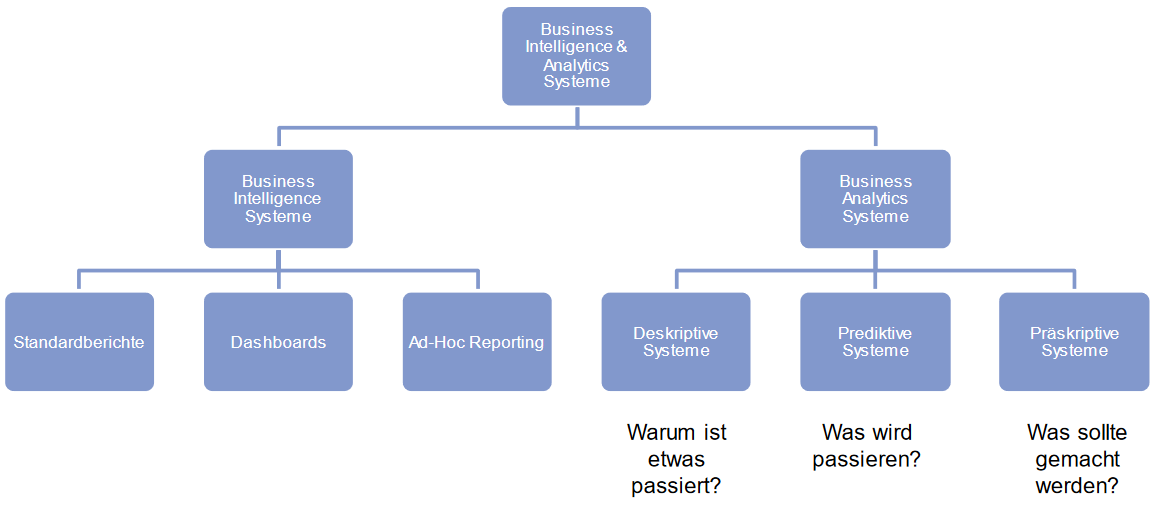
\includegraphics[width=0.9\textwidth]{images/bibas.png}
\end{center}

\textbf{Transaktionsmarketing vs. Beziehungsmarketing}:
\begin{center}
	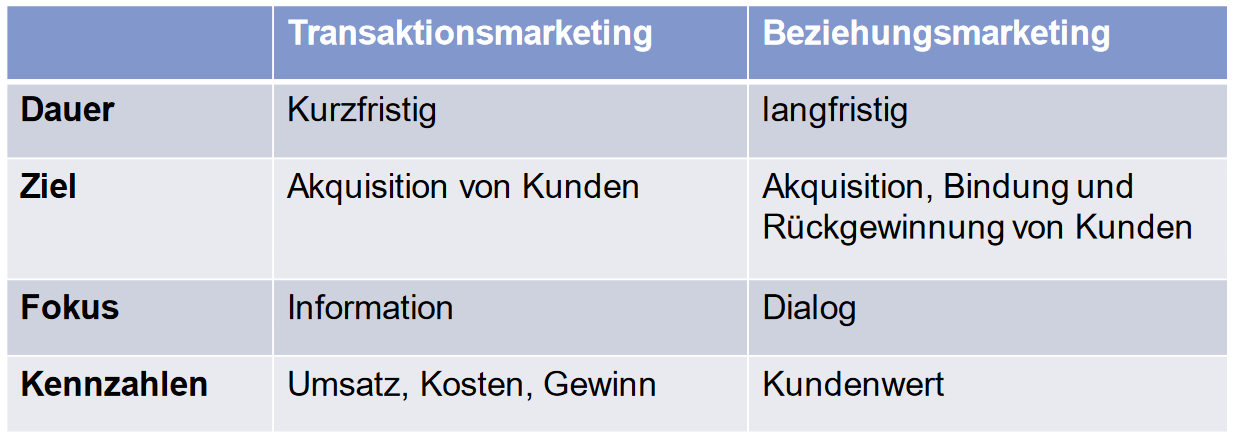
\includegraphics[width=0.8\textwidth]{images/tb.png}
\end{center}

\textbf{Kundenbeziehungsmanagementsystem} (CRM) ist ein beziehungsorientiertes, von einem Betrieb hierarchisch gesteuertes Marketinginformationssystem $\rightarrow$ \textbf{Ziel}: Aufbau von Kundenprofilen, welche Eigenschaften, die typisch für den Kunden und relevant für die Geschäftsbeziehung sind beinhalten

\pagebreak
\textbf{Operatives und Analytisches CRM}:
\begin{center}
	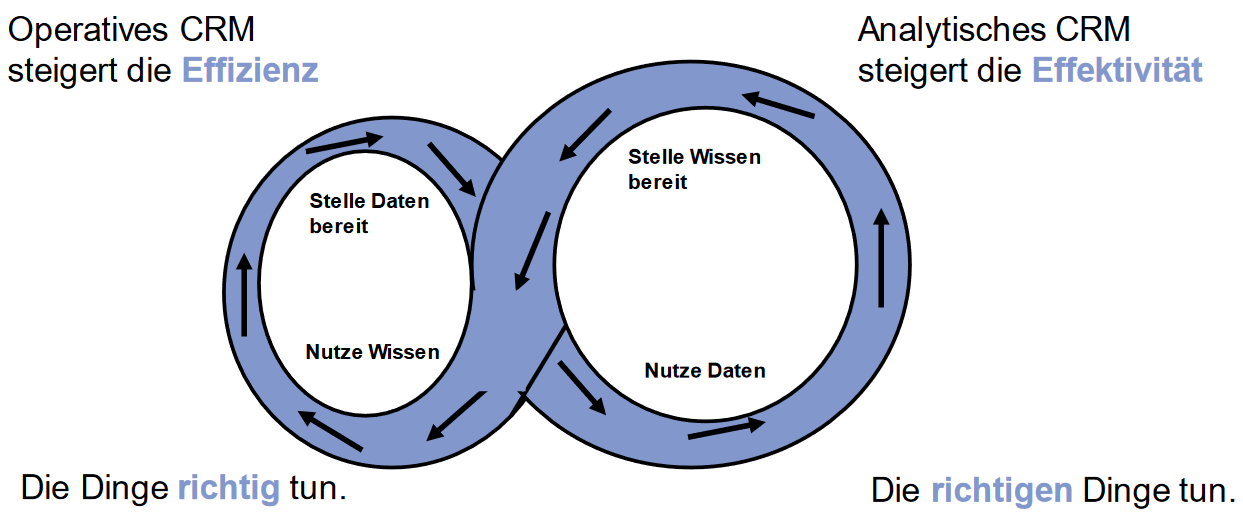
\includegraphics[width=0.6\textwidth]{images/crm.png}
\end{center}

\textbf{Architektur von CRM-Systemen}:
\begin{itemize}
	\item \textbf{Analytische CRM} fokussiert auf die Sammlung und Analyse von Kundendaten
	\item \textbf{Operative CRM} bildet kundenzentrierte Geschäftsprozesse im Bereich Vertrieb, Marketing und Kundenservice ab
	\item \textbf{Kommunikative CRM} deckt dann sämtliche Kanäle zur Kundenkommunikation
\end{itemize}

\section{KI-basierte Systeme}
\textbf{Was ist Künstliche Intelligenz?}
\begin{center}
	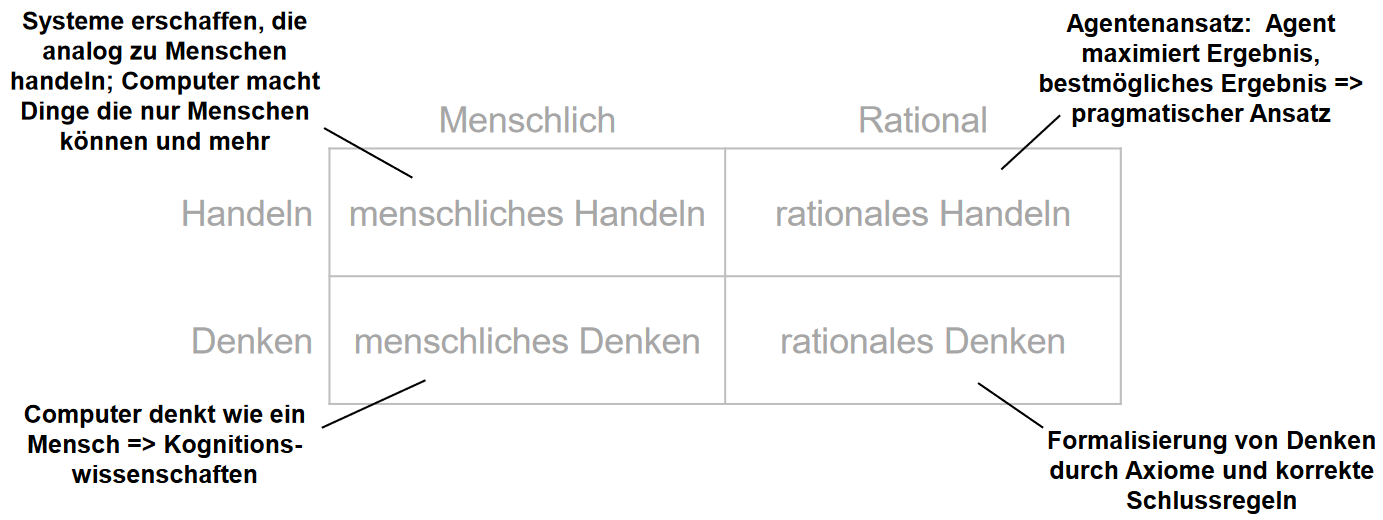
\includegraphics[width=0.8\textwidth]{images/ki.png}
\end{center}

Ein \textbf{Agent} nimmt seine Umgebung durch Sensoren wahr und verändert sie durch Effektoren

Ein \textbf{intelligenter Agent} is derjenige, der aufgrund seiner Beobachtungsfolge und seines Wissens über die Umgebung stets die optimale Aktion bzgl. eines Performanzmaß wählt
\begin{itemize}
	\item heißt \textbf{autonom}, der Agent eher aus seinen Beobachtungen lernt und nicht auf vorprogrammierte Aktionen angewiesen ist
\end{itemize}

\textbf{Key Concept: PEAS}:
\begin{itemize}
	\item \underline{P}erformance Measure: Einheit zur Definition des Erfolgs eines Agenten
	\item \underline{E}nvironment: Umgebung eines Agenten
	\item \underline{A}ctuaor: Teil des Agenten, der den Output der Handlung an die Umwelt abgibt
	\item \underline{S}ensors: Rezeptive Teile eines Agenten, die den Input für den Agenten aufnehmen
\end{itemize}

\textbf{Supervised Learning}:
\begin{itemize}
	\item Lernen mit vorklassifizierten Trainingsdaten
	\item \textbf{Ziel}: Lerne Funktion $x\rightarrow y$ um Klassifizierungen über ungesehene Daten zu treffen
\end{itemize}

\textbf{Unsupervised Learning}:
\begin{itemize}
	\item Erkennen von Mustern in unklassifizierten Daten
	\item \textbf{Ziel}: Erlernen der verborgene Struktur der Daten
\end{itemize}

\textbf{ID3 Algorithmus}:
\begin{itemize}
	\item Gehört zur Familie von Entscheidungsbaum-Lernalgorithmen, die von der Annahme ausgehen, dass Daten in Kategorien unterteilt werden können
	\item \textbf{Vorteile} von Algorithmen zum Lernen von Entscheidungsbäumen:
	\begin{itemize}
		\item Funktionieren mit kleinen Datensätzen
		\item Schnell zu trainieren
		\item Liefern Interpretierbare Ergebnisse
	\end{itemize}
	\item \textbf{Vorgehen}:
	\begin{itemize}
		\item Berechnet für jeden möglichen Split-Kandidaten ein statistisches Maß für den gegebenen Trainingsdatensatz
		\item Wählt den Split-Kandidaten, der die Beispiele im Trainingsdatensatz am besten klassifiziert
		\item Führt dies rekursiv mit den verbleibenden Split-Kandidaten durch, bis jedes Element des Trainingsdatensatzes eindeutig klassifiziert werden kann
	\end{itemize}
	
	$\rightarrow$ Greedy Top-Down-Suche, der einen kompakten, aber nicht unbedingt besten Entscheidungsbaum findet
\end{itemize}

\textbf{Informationsgewinn} gibt an, wie gut ein bestimmtes Attribut $A$ eine Menge $S$ von Trainingsbeispielen gemäß der Zielklassifizierung trennt
\begin{itemize}
	\item ID3 wählt in jedem Schritt das Attribut aus, das den Informationsgewinn für den gegebenen Satz von Trainingsbeispielen maximiert
	\item Informationsgewinn beschreibt die erwartete Verringerung der Entropie des gesamten Datensatzes durch die Aufteilung von $S$ nach dem Attribut $A$
	$$\text{Informationsgewinn}(S,A)=\text{Entropie}(S)-\sum\limits_{v\in \text{values}(A)}\frac{|Sv|}{|S|}\cdot \text{Entropie}(Sv)$$
\end{itemize}

\textbf{Entropie im Kontext von Entscheidungsbaumlernen}: 
\begin{itemize}
	\item Beim Lernen von Entscheidungsbäumen wird Entropie verwendet, um die \textbf{Unreinheit} einer Menge $S$ von Trainingsbeispielen zu berechnen
	\item Für eine binäre Klassifikation ($\oplus$ oder $\ominus$) definieren wir Entropie$(S)$ wie folgt: Sei $p_\oplus$ die relative Häufigkeit der positiven Beispiele in $S$ und $p_\ominus$ die relative Häufigkeit der negativen Beispiele in $S$:
	$$\text{Entropie}(S)=-p_\oplus \log_2 p_\oplus -p_\ominus\log_2 p_\ominus$$
	\item $S$ hat minimale Unreinheit mit Entropie $(S) = 0$ und maximale Unreinheit mit Entropie $(S) = 1$
\end{itemize}

\textbf{Informationssystem (MAT-System) mit KI Techniken}:
\begin{center}
	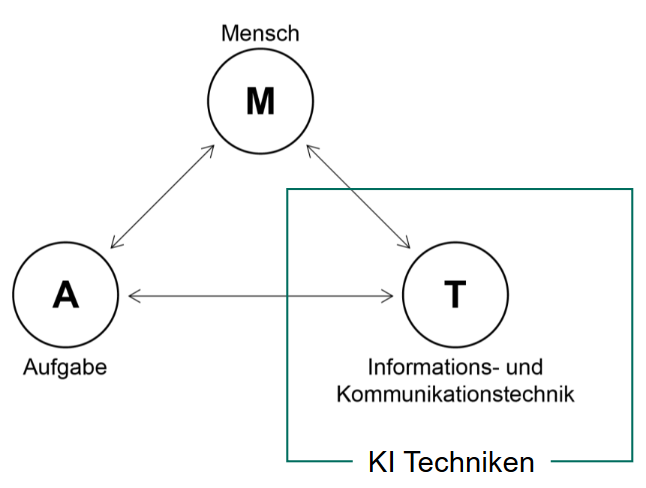
\includegraphics[width=0.5\textwidth]{images/mat-ki.png}
\end{center}
\begin{itemize}
	\item Verschiebung bei der Aufgabendurchführung von Mensch (M) zur Technik (T) $\rightarrow$ \textbf{Automatisierung}
	\item Menschen bei ihrer Aufgabendurchführung besser unterstützen $\rightarrow$ \textbf{Augmentation}
\end{itemize}

\textbf{Konversationsagenten} sind softwarebasierte Systeme, die für die Interaktion mit Nutzern unter Verwendung natürlicher Sprache konzipiert sind

\textbf{Nutzeradaptive Systeme} nutzen Kontextinformation um Adaptation zu realisieren. Biosignale bieten reichhaltige Information über den Nutzerkontext

\pagebreak
\textbf{Potenziale und Risiken von KI}:
\begin{center}
	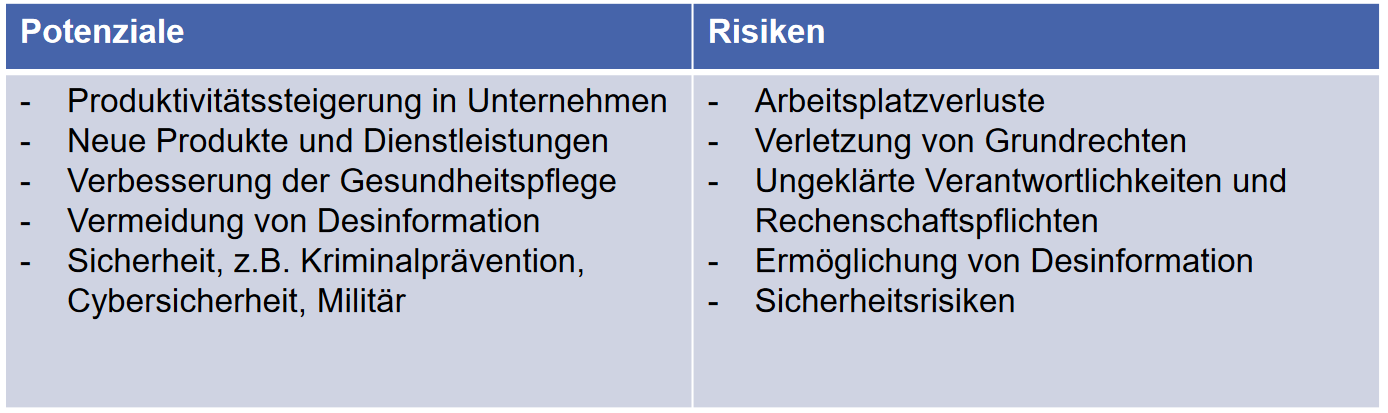
\includegraphics[width=0.8\textwidth]{images/ki-risc.png}
\end{center}

\textbf{Ethische Grundsätze und Anforderungen}:
\begin{itemize}
	\item 4 ethische Grundsätze:
	\begin{enumerate}
		\item Achtung der menschlichen Autonomie
		\item Schadensverhütung
		\item Fairness
		\item Erklärbarkeit
	\end{enumerate}
	\item 7 Anforderungen:
	\begin{enumerate}
		\item Vorrang menschlichen Handelns und menschliche Aufsicht
		\item technische Robustheit und Sicherheit
		\item Schutz der Privatsphäre und Datenqualitätsmanagement
		\item Transparenz
		\item Vielfalt, Nichtdiskriminierung und Fairness
		\item gesellschaftliches und ökologisches Wohlergehen sowie
		\item Rechenschaftspflicht
	\end{enumerate}
\end{itemize}

\section{Digitale Plattformen}

A \textbf{Platform} is a business model that creates value by facilitating exchanges between two or more interdependent groups, usually consumers and producers

\textbf{Netzwerkeffekte}:
\begin{itemize}
	\item \textbf{Externe Effekte}: Beschreiben eine Situation, in welcher der Konsum eines Individuums direkt den Nutzen eines anderen Individuums beeinflusst
	\item \textbf{Netzwerkeffekte bzw. Netzwerkexternalitäten}: Nutzen eines Gutes hängt von der Anzahl weiterer Nutzer ab
	\item \textbf{Direkte Netzwerkeffekte}: Nutzen der Individuen hängt direkt von der Anzahl der Nutzer ab
	\item \textbf{Indirekte Netzwerkeffekte}: Basieren auf unterschiedlichen komplementären Gütern
\end{itemize}

\textbf{Märkte mit Netzwerkeffekten}:
\begin{center}
	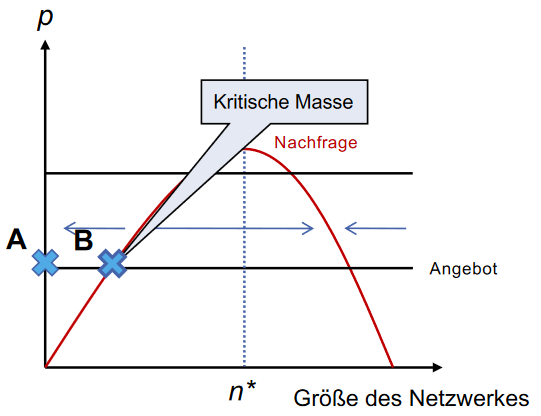
\includegraphics[width=0.4\textwidth]{images/netzwerkeffekte.png}
\end{center}
\begin{itemize}
	\item Größeres Netzwerk ($n>n^*$): je größer das Netzwerk, desto geringer ist die Zahlungsbereitschaft eines zusätzlichen Teilnehmers am Netzwerk
	\item Kleines Netzwerk ($n<n^*$): je kleiner das Netzwerk, desto geringer ist der	individuelle Nutzen, desto geringer ist die Nachfrage 
	\item Übersteigt die Nachfrage das Angebot, d.h. die Zahlungsbereitschaft übersteigt den Preis, so expandiert der Markt und umgekehrt
	\item $A$ ist ein stabiles low-level Gleichgewicht, niemand konsumiert das Gut bzw. niemand nimmt am Netzwerk teil
	\item Wird \textbf{kritische Netzwerkgröße} $B$ überschritten, wächst das Netzwerk stark an
\end{itemize}

\textbf{Klassifikation von Auktionen}: 
\begin{center}
	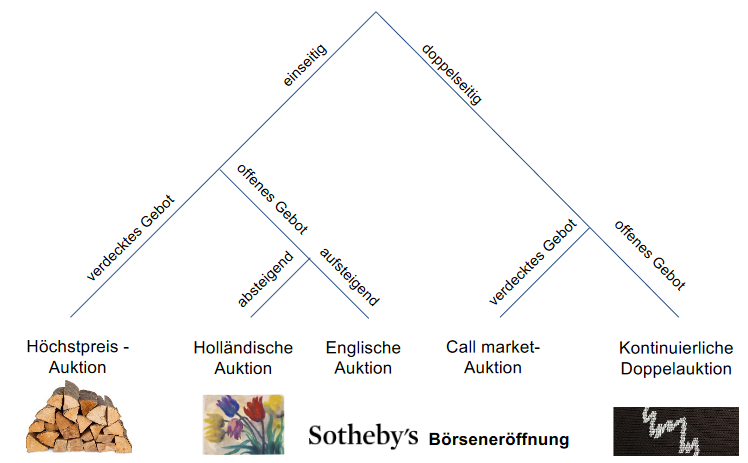
\includegraphics[width=0.7\textwidth]{images/auktionsformate.png}
\end{center}

\pagebreak
\textbf{Auktionsformate}:
\begin{center}
	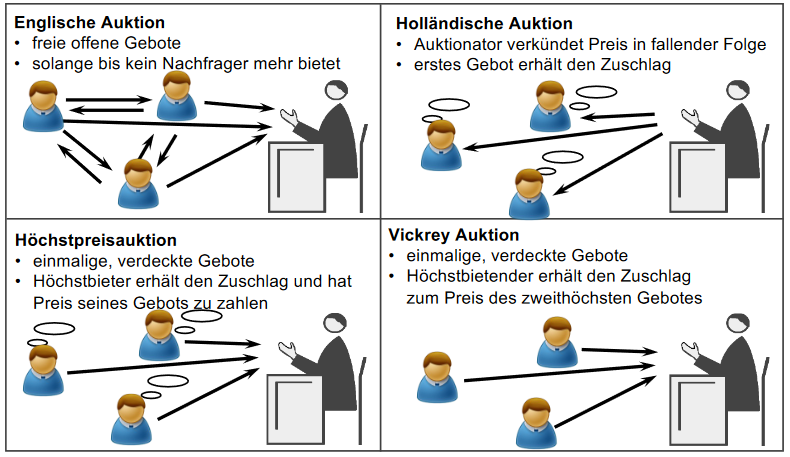
\includegraphics[width=0.7\textwidth]{images/auktionsformate-2.png}
\end{center}

\textbf{SIEHE VL8/F141-142 BERECHNUNGEN!}

\section{Interaktive Systeme}

\textbf{Interaktionstechnik} beschreibt IKT, welche Nutzern ermöglicht im IS für die Aufgabendurchführung zu interagieren. Es wird zwischen Eingabe- und Ausgabe-Interaktionstechnik unterschieden.

\textbf{Modalität} beschreibt die Art des Kommunikationskanals welcher verwendet wird um Information zu erfassen oder vermitteln
\begin{itemize}
	\item \textbf{Eingabemodalitäten}: Art und Weise, in der Benutzer dem System über ihre Effektoren Input geben
	\item \textbf{Ausgabemodalitäten}: Art und Weise, in der Benutzer die Ausgabe über ihre fünf Sinne wahrnehmen
\end{itemize}

Interaktionsparadigmen entwickeln sich rasant $\rightarrow$ Mehr Nutzer, Mehr Geräte, Mehr Interaktionen

\textbf{Barrierefreiheit} ist das Ausmaß, in dem ein interaktives System es den
Nutzern ermöglicht unabhängig von ihrem Sehvermögen, Gehör, Geschicklichkeit, Kognition, körperlicher Mobilität usw. zu interagieren

\textbf{Gebrauchstauglichkeit} ist das Ausmaß, in dem ein Produkt durch bestimmte Nutzer in einem bestimmten Nutzungskontext genutzt werden kann, um bestimmte Ziele effektiv, effizient und zufriedenstellend zu erreichen

\textbf{Leitkriterien für die Usability einer Software}:
\begin{itemize}
	\item Effektivität: Genauigkeit und Vollständigkeit, mit der Benutzer ein bestimmtes Ziel erreicht
	\item Effizienz: Der im Verhältnis zur Genauigkeit und Vollständigkeit eingesetzte Aufwand, mit dem Benutzer ein bestimmtes Ziel erreicht
	\item Zufriedenstellung: Freiheit von Beeinträchtigung und positive Einstellung gegenüber der Nutzung des Produkts
\end{itemize}

\textbf{User Experience}: Wahrnehmungen und Reaktionen eines Benutzers, die sich aus der Nutzung oder der erwarteten Nutzung eines interaktiven Systems ergeben

\textbf{Beziehung zwischen Usability und User Experience}:
Usability ist Effektivität, Effizienz und Zufriedenheit während der tatsächlichen Nutzung, wohingegen sich die User Experience auf allgemeine Wahrnehmungen und Reaktionen während der erwarteten Nutzung, der tatsächlichen Nutzung und nach der Nutzung bezieht

\textbf{Gruppen} sind eine Sammlung von Individuen, die in ihren Aufgaben voneinander abhängig sind, die die Verantwortung für die Ergebnisse teilen, sich selbst und von anderen als intakte soziale Einheit betrachtet werden, die in ein oder mehrere größere soziale Systeme eingebettet sind, und die ihre Beziehungen über Organisationsgrenzen hinweg verwalten

\textbf{Teams} und \textbf{Communities} grenzen sich voneinander ab durch den Grad der Formalität, der Kommunikation und dem Fokus der Zusammenarbeit

\textbf{Soziale Interaktion} bezeichnet das Geschehen zwischen Personen, die aufeinander reagieren, miteinander umgehen, einander beeinflussen und steuern, z.B. Austausch, Wettbewerb, Koordination, Kooperation oder Konflikt

\textbf{Koordination} ist das Management von Abhängigkeiten zwischen Aktivitäten

\textbf{CSCW (Computer Supported Cooperative Work)} untersucht und gestaltet computergestütztes kooperatives Arbeiten, in welcher Informationstechnologie verwendet wird, um soziale Interaktion in Gruppen zu ermöglichen, um gemeinsam Ergebnisse zu erzielen

\textbf{Social Computing} bezieht sich auf Systeme, die das Sammeln, Darstellen, Verarbeiten, Verwenden und Verbreiten von Informationen unterstützen, die über soziale Kollektive verteilt sind

\textbf{Klassifikation von CSCW Systemen nach Zeit und Ort}:
\begin{center}
	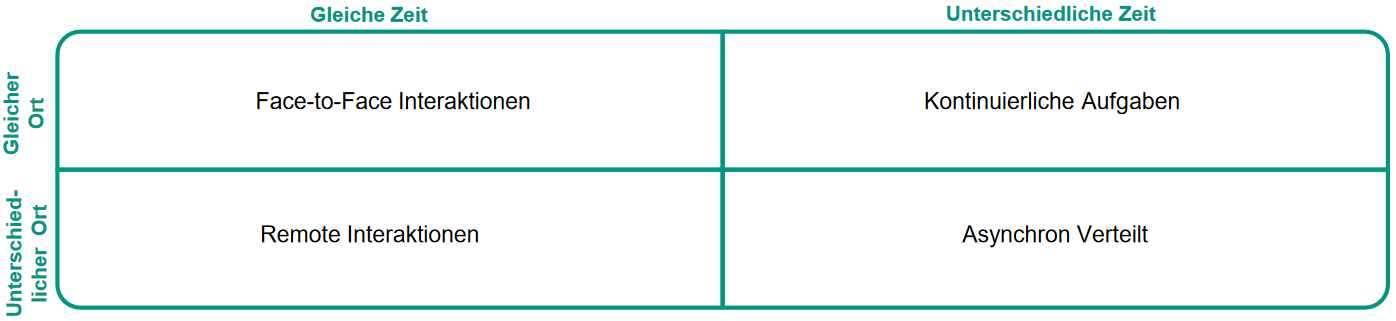
\includegraphics[width=0.9\textwidth]{images/cscw.png}
\end{center}

\pagebreak
\textbf{Klassische Erklärungsmodelle für Akzeptanz und Nutzung von Systemen}:
\begin{center}
	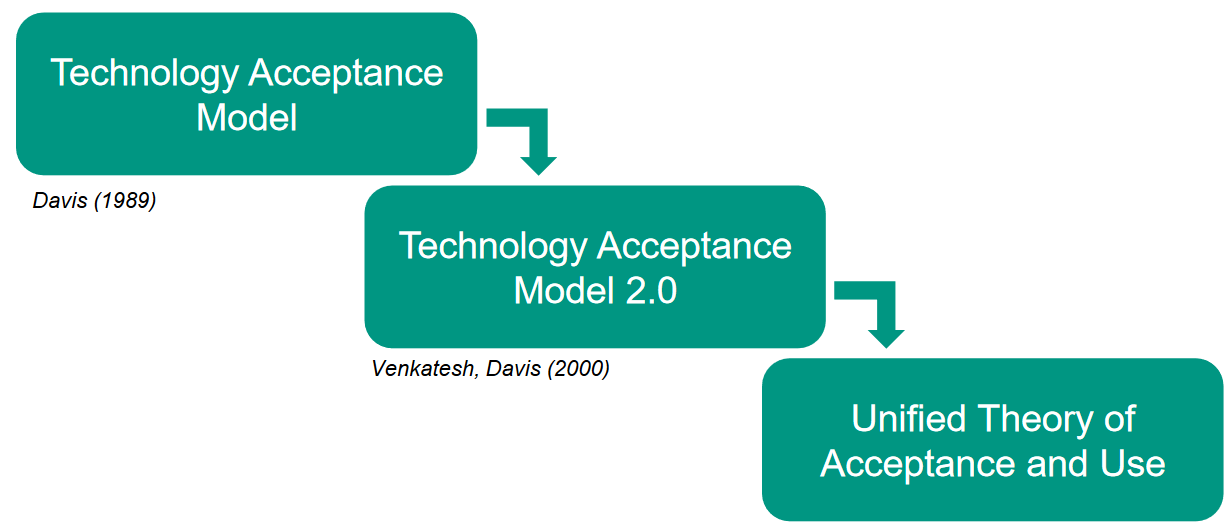
\includegraphics[width=0.5\textwidth]{images/e-modelle.png}
\end{center}

\textbf{Technology Acceptance Model (TAM)}:
\begin{center}
	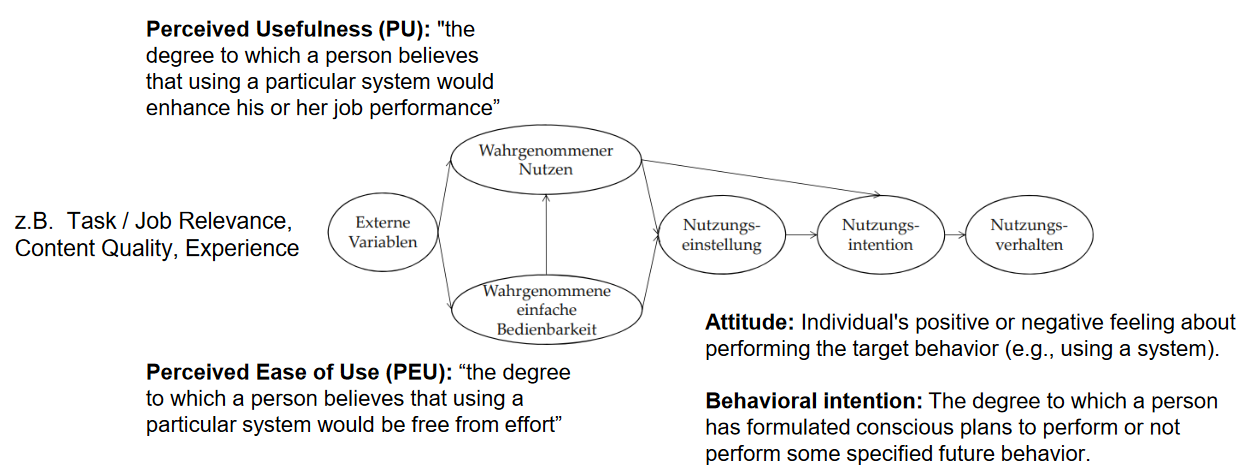
\includegraphics[width=0.9\textwidth]{images/tam.png}
\end{center}

\textbf{Unified Theory of Acceptance and Use of Technology (UTAUT)}:
\begin{center}
	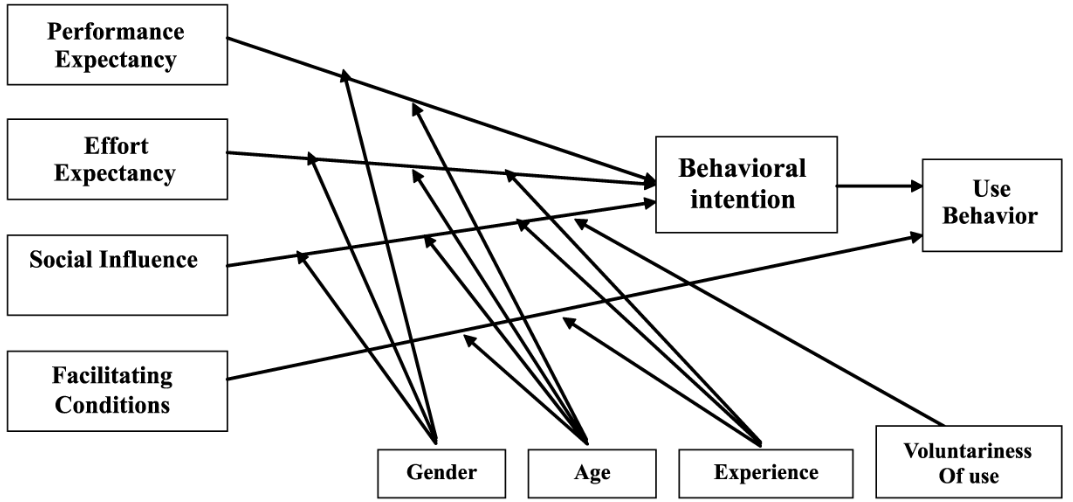
\includegraphics[width=0.7\textwidth]{images/utaut.png}
\end{center}

\textbf{Nutzung} ist die Anwendung eines Systems durch ein Individuum zur Ausführung einer Aufgabe

\textbf{Effektive Nutzung}: Individuen nutzen ein System in einer Art und Weise, so dass die Zielerreichung steigt, die mit der Nutzung des Systems verfolgt wird